% šablona na pro bakalářskou práci na FAI UTB
% šablona je úpravou původní šablony pro FAI UTB
% =======================================================
% verze 0.9.5 (10. říjen 2005)
% autor: Ing. Jozef Říha ()
% některé komentáře převzaty z dokumentu Ivana Pomykacze
% =======================================================
% upravil Martin Zajíc
% šablona je upravena aby šla bez problému přeložit pomocí TeXlive a překladače XeLaTeX
% XeLaTex také řeší neduhy spojené s kódováním českých znaků a jejich kopírování z PDF dokumnetu
\documentclass[a4paper,12pt]{article}
\usepackage{xltxtra}
\usepackage[czech]{babel}
\usepackage{listings}
\usepackage{indentfirst}
\usepackage{color}
\usepackage[svgnames]{xcolor} 
\usepackage{colortbl}
\usepackage{array}
\usepackage{graphicx}
\usepackage{amsmath}
\usepackage{fancyhdr}
\usepackage{fancyvrb}
\usepackage{fancybox,calc} 
\usepackage{hyperref}
\usepackage{multirow}
\usepackage{tocloft}
\usepackage{textcase}
\usepackage{ifthen}
\usepackage{setspace}
\usepackage{ccaption}
\usepackage{sectsty}
\usepackage{wrapfig}
%\usepackage[srcstyle=leftnumhang,linenumbersep={\ }]{examplep}
% ************************ NASTAVENÍ AUTORA A NÁZVU DOKUMENTU ************************
\newcommand{\rok}{2014}
\newcommand{\jmeno}{Martin Zajíc}
\newcommand{\typprace}{Diplomová práce}
\newcommand{\predmet}{Informační systém knihkupectví}
\newcommand{\predmeten}{přeložit}
% ************************ NASTAVENÍ TISKOVÉHO ZRCADLA ************************
\textheight=248mm
\textwidth=155mm
\voffset=-1.61cm
\oddsidemargin=0.96cm
\evensidemargin=0.96cm

% nastavení záhlaví
\headheight=0.5cm
\headsep=1cm

% nastavení zápatí
\footskip=1ex
\rhead{\thepage}
\cfoot{}
% "vypnout" poznámky na okrajích
\marginparpush=0mm
\marginparwidth=0mm
\marginparsep=0mm

\pagestyle{fancy}
% ****************** NASTAVENÍ HYPERPREF (BAREV ODKAZŮ, PDF DOKUMENTU) **************
\hypersetup{
    pdftoolbar=true,        % show Acrobat’s toolbar?
    pdfmenubar=true,        % show Acrobat’s menu?
    pdftitle={\typprace~-~\predmet },    % title
    pdfauthor={\jmeno},     % author
    pdfsubject={\predmet},   % subject of the document
    pdfcreator={\jmeno},   % creator of the document
    colorlinks=true,       % false: boxed links; true: colored links
    linkcolor=black,          % color of internal links
    citecolor=black,        % color of links to bibliography
    filecolor=black,      % color of file links
    urlcolor=black           % color of external links
}

% ****************** NASTAVENÍ PÍSMA, ODSTAVCE, ROVNIC, POZNÁMEK **************
\parindent=0em
\def\thefootnote{\arabic{footnote})}	% poznámka pod čarou se závorkou
\onehalfspacing % nastavím řádkování tímto způsobem nebo \renewcommand{\baselinestretch}{1.5} ??
\setlength{\parskip}{3pt}		% vertikální mezera mezi nadpisy
% *************************** NASTAVENÍ ČÍTAČŮ	 ********************************
\setcounter{tocdepth}{3} % do obsahu se ukládají pouze první dvě úrovně kapitol

% *************************** UŽIVATELSKÉ STYLY *******************************
\newcommand{\nn}[1]{\clearpage\section*{\texorpdfstring{\uppercase{#1}}{#1}}\addcontentsline{toc}{section}{\uppercase{#1}}}% styl nn = nečíslovaný nadpis (je vysázený v obsahu)
\newcommand{\nm}[1]{\clearpage\section*{\uppercase{#1}}}	% definujeme styl nm = nečíslovaný nadpis (není vysázený v obsahu)
\newcommand{\nmm}[1]{\section*{#1}} % definujeme styl nmm = nečíslovaný nadpis (není vysázený v obsahu) malými písmeny bez clearpage
\newcommand{\nns}[1]{\section*{\uppercase{#1}}}		% definujeme styl ns = nečíslovaný nadpis na stejné stránce (není vysázený v obsahu)
\newcommand{\sectionV}[1]{\section{\uppercase{#1}}}	%nadpis1 (section) velkým
%\renewcommand{\section}[1]{\section{\uppercase{#1}}}
\newcommand{\upc}[1]{\uppercase{#1}} %zjednodušení pro velká písmena
\newcommand{\odkazNaKapitolu}[1]{(viz.~kapitola~\ref{#1}/s\pageref{#1})}
\newcommand{\odkazNaObrazek}[1]{(viz.~obr.~\ref{#1}/s\pageref{#1})}

\newcommand{\nadpis}[1]{%nadpis pod kterym je vertikalni mezera
	\vspace{4 mm}
	\textbf{#1}\\
	\vspace{4 mm}
	}

\newcommand{\obr}[3]{% styl \obr pro obrázky
	\begin{figure}[h]
	\center\includegraphics[scale=#2]{#1}
	\caption{#3}
	\end{figure}
	}

\newcommand{\ofZadani}[2]{% styl \obr pro obrázky
	\begin{figure}[h]
	\center\includegraphics[width=500pt,height=700pt]{#1}
	%\caption{#2}
	\end{figure}
	}

\newcommand{\tab}[3]{% styl \tab pro tabulky
	\begin{table}[h]
	\caption{#1}
	\begin{center}
	\begin{tabular}{#2}
	#3
	\end{tabular}
	\end{center}
	\end{table}
	}

\newcommand{\tabpri}[3]{% styl \tabpri pro tabulky v příloze
	\begin{table}[h]
	\begin{center}
	#1
	\end{center}
	\begin{center}
	\begin{tabular}{#2}
	#3
	\end{tabular}
	\end{center}
	\end{table}
	}

\newcommand{\rov}[2][chybějici rovnice]{% styl \rov pro rovnice
	\begin{equation}
	#2
	\label{#1}
	\end{equation}
	}
	
\newcommand{\seznamobr}{% příkaz \seznamobr pro vysázení seznamu obrázků
	\addcontentsline{toc}{section}{\listfigurename}
	\clearpage
	\listoffigures
	\clearpage
	}

\newcommand{\seznamtab}{% příkaz \seznamtab pro vysázení seznamu obrázků
	\addcontentsline{toc}{section}{\listtablename}
	\clearpage
	\listoftables
	\clearpage
	}
	
\newcommand{\seznamlit}[1]{% příkaz \seznamlit pro vysázení seznamu literatury
	\addcontentsline{toc}{section}{\refname}
	\begin{thebibliography}{10}
	#1
	\end{thebibliography}}
	
\newcommand{\seznamzkr}{% příkaz \seznamzkr pro přípravu seznamu použitých zkratek a symbolů
	\nn{Seznam použitých symbolů a zkratek}
	}
	
\newcommand{\obsah}{% \obsah vysází obsah v daném místě
	\clearpage
	\thispagestyle{empty}
	\tableofcontents
	\clearpage
	\pagestyle{fancy}
	}

\renewcommand{\b}[1]{\textbf{#1}} % \b = tučně
\newcommand{\bi}[1]{\textbf{\textit{#1}}}	% \bi = tučná kurzíva
\renewcommand{\it}[1]{\textit{#1}}		% \it = kurzíva
	
% ******* NASTAVENÍ ZOBRAZENÍ PŘÍLOH -- SEZNAM, ČÍSLOVÁNÍ, VLASTNÍ STYL *******
\makeatletter % tímto příkazem dávám najevo, že budu editovat přímo příkazy ze šablony

% definice seznamu příloh - příkaz \listofappendices
\newcommand{\listofappendices}{%
	\newpage
	\setcounter{section}{0}
	\nn{Seznam příloh}
	\@restonecolfalse\if@twocolumn\@restonecoltrue\onecolumn\fi
	\@mkboth{LIST OF APPENDICES}{LIST OF APPENDICES}
	\@starttoc{loa}\if@restonecol\twocolumn\fi
	\pagestyle{empty}
	\thispagestyle{fancy}
	}

\def\ext@appendix{loa}
\def\tocname{loa}

% definice příkazu \priloha{nazev prilohy} pro vložení nové přílohy
\newcommand{\priloha}[1]{
	\clearpage
	\refstepcounter{section}
	\addtocontents{loa}{\protect\makebox[1.5cm][l]{P \@Roman\c@section.} #1\newline}
{\bf PŘÍLOHA P \@Roman\c@section. \uppercase{#1}}\par\vspace{0.5cm}}

% v obsahu nastavím VELKÉ PÍSMENA pro styl část
\renewcommand{\part}[1]{
	\refstepcounter{part}
	\addcontentsline{toc}{section}{\thepart~~\uppercase{#1}}%
\clearpage
\normalfont
	\vspace*{9cm}
	\begin{center}\huge \bfseries\thepart. \uppercase{#1}\end{center}%
	\markboth{}{}\par
\nobreak
\clearpage	
}
% *******************Barevný code *******************
\definecolor{codeback}{gray}{0.8} %barva pozadi

\newenvironment{codeframe}{% 
  \begin{Sbox} 
    \begin{minipage} 
      {\columnwidth-\leftmargin-\rightmargin-2\fboxsep-2\fboxrule-4pt} 
}{% 

  \end{minipage} 
  \end{Sbox} 
  \begin{center} 
    \fcolorbox{black}{codeback}{\TheSbox} 
  \end{center} 
} 

% *************** NASTAVENÍ FORMÁTU ČÍSLOVÁNÍ OBRÁZKŮ A TABULEK ***************
\def\thefigure{\arabic{figure}}      % číslování obrázků typu (y)
\def\thetable{\arabic{table}}        % číslování tabulek typu (y)
\captiondelim{. } % změníme dvoutečku za Obr/Tab za tečku

% ***************************** VYNULOVÁNÍ ČÍTAČŮ *****************************
\@addtoreset{table}{section}    % vynulování čítače
%\@addtoreset{figure}{section}   % vynulování čítače
\@addtoreset{footnote}{section} % vynulování čítače
	
\makeatother % a to je ukončení \makeatletter

% ************* ÚPRAVA VZHLEDU OBSAHU, SEZNAMU OBRÁZKÙ A TABULEK **************
% nastavení vertikální mezery před stylem část, nadpis 1--3
\setlength{\cftbeforepartskip}{3pt}
\setlength{\cftbeforesecskip}{3pt}
\setlength{\cftbeforesubsecskip}{3pt}
\setlength{\cftbeforesubsubsecskip}{0cm}
% odsazení zleva pro styl část, nadpis 1--3
\setlength{\cftpartindent}{0cm}
\setlength{\cftsecindent}{0cm}
\setlength{\cftsubsecindent}{0cm}
\setlength{\cftsubsubsecindent}{0cm}
% nastavení fontu pro styl část, nadpis 1--3
\renewcommand{\cftpartfont}{\small\bfseries}
\renewcommand{\cftsecfont}{\small\bfseries}
\renewcommand{\cftsubsecfont}{\scshape}
\renewcommand{\cftsubsubsecfont}{}
% odsazení čísla a textu titulku pro styl část, nadpis 1--3
\cftsetindents{part}{0cm}{1cm}
\cftsetindents{sec}{0cm}{1cm}
\cftsetindents{subsec}{1cm}{1.5cm}
\cftsetindents{subsubsec}{1.2cm}{1.7cm}
\cftsetindents{fig}{0cm}{1.5cm}
\cftsetindents{tab}{0cm}{1.5cm}
% nastavení vodící čáry pro styl část, nadpis 1--3, obrázky a tabulky
\renewcommand{\cftdot}{\ensuremath{.}} % tímto příkazem lze změnit vodící tečky v obsahu na jiný znak
\renewcommand{\cftpartleader}{\cftdotfill{0.3}}
\renewcommand{\cftsecleader}{\cftdotfill{0.3}}
\renewcommand{\cftsubsecleader}{\cftdotfill{0.3}}
\renewcommand{\cftsubsubsecleader}{\cftdotfill{0.3}}
\renewcommand{\cftfigleader}{\cftdotfill{0.3}}
\renewcommand{\cfttableader}{\cftdotfill{0.3}}
% změna fontu pro text "Obsah", "Seznam obrázků" a "Seznam tabulek"
\renewcommand{\cfttoctitlefont}{\normalsize\bfseries\thispagestyle{empty}}
\renewcommand{\cftloftitlefont}{\normalsize\bfseries\thispagestyle{fancy}}
\renewcommand{\cftlottitlefont}{\normalsize\bfseries\thispagestyle{fancy}}
\renewcommand{\cftfigpresnum}{Obr. }
\renewcommand{\cftfigaftersnum}{.}
\renewcommand{\cfttabpresnum}{Tab. }
\renewcommand{\cfttabaftersnum}{.}

% ************************ NASTAVENÍ FONTU PRO NADPISY ************************
\sectionfont{\normalsize}
\subsectionfont{\normalsize\bfseries} 
\subsubsectionfont{\normalsize\bfseries}
\paragraphfont{\small\bf}
% definice nového stylu \comment -- komentář k šabloně
%\newcommand{\comment}[1]{\color{red}#1\color{black}}

% ****************************** KONEC PREAMBULE ******************************
\begin{document}
% ****************************** Vlastní definice ******************************
% ********* musí být na začátku dokumnetu v preambuli nefungují ****************
\renewcommand{\refname}{\texorpdfstring{\uppercase{Seznam použité literatury}}{Seznam použité literatury}}
\renewcommand*{\listfigurename}{\texorpdfstring{\uppercase{Seznam obrázků}}{Seznam obrázků}}
\renewcommand{\contentsname}{\texorpdfstring{\uppercase{Obsah}}{Obsah}}
\renewcommand*{\listtablename}{\texorpdfstring{\uppercase{Seznam tabulek}}{Seznam tabulek}}
\renewcommand*{\tablename}{Tab.}
\renewcommand\figurename{Obr.}
%********************************* Hlavička ************************************
\lhead{\b{UTB ve Zlíně, Fakulta aplikované informatiky}}

\thispagestyle{empty}
\voffset=-2.01cm\evensidemargin=0pt\oddsidemargin=0cm\parindent=0pt\headsep=0pt\headheight=0pt\parskip=0pt\textheight=272mm\textwidth=200mm
\renewcommand{\baselinestretch}{0}
%********************************* Úvodní stránka s logem fakulty ********************
\setlength{\unitlength}{1mm}
\begin{picture}(-10,8)
\put(0,-50){\makebox(170,50){}}
%*******************************Uvodni stranka z nazvem prace na dva radky*********
%\put(0,-100){\makebox(170,50){\fontsize{24}{1}\b{\textsf{Zálohovací server založený na}}}}
%\put(0,-110){\makebox(170,50){\fontsize{24}{1}\b{\textsf{GNU/Linux Debian}}}}
%\put(0,-130){\makebox(170,50){\fontsize{20}{1}\b{\textsf{Backup server based on GNU/Linux Debian}}}}
%\put(0,-150){\makebox(170,25){\fontsize{20}{1}\b{\textsf{\jmeno}}}}
%*******************************konec uvodni stranka na dva radky***********************
\put(0,-115){\makebox(170,50){\fontsize{24}{1}\b{\textsf{\predmet}}}}
\put(0,-130){\makebox(170,50){\fontsize{22}{1}\b{\textsf{\predmeten}}}}
\put(0,-150){\makebox(170,25){\fontsize{20}{1}\b{\textsf{\jmeno}}}}
\put(82.2,-223.3){\makebox(84,16.4){
\includegraphics[width=84mm]{fai_logo_cz.png}}}
\put(0,-205){\linethickness{1pt}\line(1,0){170}}
\put(4,-215){\makebox(69.5,4.5)[l]{\noindent\fontsize{16}{1}\b{\textsf{\typprace}}}}
\put(4,-220){\makebox(69.5,4.5)[l]{\noindent\fontsize{16}{1}\b{\textsf{\rok}}}}
\put(0,-225){\linethickness{1pt}\line(1,0){170}}
\put(75,-223.3){\linethickness{1pt}\line(0,1){16.4}}
\end{picture}
%********************************* nascanované zadání ************************************
\clearpage
\thispagestyle{empty}
\ofZadani{./img/ofZadani/ofZadaniStr1.png}{Oficiální zadání bakalářské práce strana 1}
\clearpage
\thispagestyle{empty}
\ofZadani{./img/ofZadani/ofZadaniStr2.png}{Oficiální zadání bakalářské práce strana 2}
%********************************* Abstrakt ************************************
\clearpage
\thispagestyle{empty}
\voffset=-1.61cm\evensidemargin=0.96cm\oddsidemargin=0.96cm\headsep=1cm\headheight=0.5cm\setlength{\parskip}{3pt}\textheight=248mm\textwidth=155mm
\nm{\uppercase{Abstrakt - smazat}}
\vspace{1cm}
Tato bakalářská práce v teoretické části definuje základní pojmy, jako jsou Linux, dále pak linuxové distribuce, jazyk BASH, zabezpečení operačního systému Linux a~LiveCD. Úvodní část je věnována informacím o~systému Linux a~distribuci Linux From Scratch. Dále pak obsahuje stručný úvod do jazyka BASH a~kompilaci zdrojových kódů včetně možností sestavení Linuxových distribucí. Na závěr teoretické části je popsáno zabezpečení Linuxu, hodnocení bezpečnosti Software a tvorba LiveCD.\\

V praktické části je rozebrána struktura scriptů a~funkce vytvořené v~jazyce BASH. Dále je uveden návod~na sestavení distribuce LFS pomocí vytvořených skriptů. A~na~závěr uvedeny zdroje pomoci při chybách v~kompilaci a~možnosti zlepšení skriptů.
\vspace{1cm}

\emph{Klíčová slova:} Linux, distribuce, BASH, LFS, LiveCD, bezpečnost Linuxu, kompilace, DAC, MAC
\vspace{2cm}

\nns{\uppercase{Abstract  - smazat}}
This bachelor work includes the terms such as~Linux in~it's~theoretical part. Further, the terms such as~Linux distribution, BASH language, operating system security, and~LiveCD. The~introductory part is~dedicated to~the~information about the~Linux system and~Linux From Scratch distribution. Then it~also includes brief introduction to~the~BASH language and~the~source code compilation, including the~possibility to~compile Linux distributions. At~the~end of~the~theoretical part, there is~described Linux security, the~evaluation of~Software security and~the~LiveCD creation.\\

In the practical part, there is~analysed the~script structure and~the~functions written in~BASH language. Next, there is~the~manual for~compiling LFS distributions using the~generated scripts. And~at~the~end of~this part, there are~mentioned resources to~compilation errors and~the possibilities of~script improvement.
\vspace{1cm}

\emph{Keywords:} Linux, distribution, BASH, LFS, LiveCD, Linux security, compilation, DAC, MAC
%********************************* poděkování, motto, úryvky knih, básní atp. ************************************
\clearpage
\thispagestyle{empty}
 - smazat
Chtěl bych poděkovat především vedoucímu mé bakalářské práce, panu doc. Ing.~Martinu~Syslovy,~Ph.D., za jeho cenné rady a~připomínky.
Dále bych chtěl poděkovat celé mojí rodině za její obrovskou podporu během celého mého studia a~také mým přátelům, se kterými jsem prožil tři roky studia na Univerzitě Tomáše Bati.

\vspace{3cm}
"Nejlepší knihy jsou takové, které člověku říkají, co už sám ví."\\

\hspace{9cm}GEORGE ORWELL
%********************************* Prohlášení ************************************
\clearpage
\thispagestyle{empty}
\clearpage
\nmm{Prohlašuji, že}
\begin{itemize}\fontsize{10}{1}
\normalsize
\item beru na vědomí, že odevzdáním bakalářské práce souhlasím se zveřejněním své práce podle zákona č. 111/1998 Sb. o vysokých školách a o změně a doplnění dalších zákonů (zákon o vysokých školách), ve znění pozdějších právních předpisů, bez ohledu na výsledek obhajoby;
\item beru na vědomí, že bakalářská práce bude uložena v elektronické podobě v univerzitním informačním systému dostupná k prezenčnímu nahlédnutí, že jeden výtisk bakalářské práce bude uložen v příruční knihovně Fakulty aplikované informatiky Univerzity Tomáše Bati ve Zlíně a jeden výtisk bude uložen u vedoucího práce; 
\item byl/a jsem seznámen/a s tím, že na moji bakalářskou práci se plně vztahuje zákon č. 121/2000 Sb. o právu autorském, o právech souvisejících s právem autorským a o změně některých zákonů (autorský zákon) ve znění pozdějších právních předpisů, zejm. § 35 odst. 3;
\item beru na vědomí, že podle § 60 odst. 1 autorského zákona má UTB ve Zlíně právo na uzavření licenční smlouvy o užití školního díla v rozsahu § 12 odst. 4 autorského zákona;
\item beru na vědomí, že podle § 60 odst. 2 a 3 autorského zákona mohu užít své dílo –bakalářskou práci nebo poskytnout licenci k jejímu využití jen s předchozím písemným souhlasem Univerzity Tomáše Bati ve Zlíně, která je oprávněna v takovém případě ode mne požadovat přiměřený příspěvek na úhradu nákladů, které byly Univerzitou Tomáše Bati ve Zlíně na vytvoření díla vynaloženy (až do jejich skutečné výše);
\item beru na vědomí, že pokud bylo k~vypracování bakalářské práce využito softwaru poskytnutého Univerzitou Tomáše Bati ve Zlíně nebo jinými subjekty pouze ke studijním a~výzkumným účelům (tedy pouze k~nekomerčnímu využití), nelze výsledky bakalářské práce využít ke komerčním účelům;
\item beru na vědomí, že pokud je výstupem bakalářské práce jakýkoliv softwarový produkt, považují se za součást práce rovněž i~zdrojové kódy, popř. soubory, ze kterých se projekt skládá. Neodevzdání této součásti může být důvodem k~neobhájení práce.
\end{itemize}
\nmm{Prohlašuji,}
\begin{itemize}
 \normalsize
\item že jsem na bakalářské práci pracoval samostatně a použitou literaturu jsem citoval. V případě publikace výsledků budu uveden jako spoluautor.
\item že odevzdaná verze bakalářské práce a verze elektronická nahraná do IS/STAG jsou totožné.
\end{itemize}
\vspace{1cm}
\begin{tabular}{lc}
Ve Zlíně &\hspace{9cm} .......................\\
~ &\hspace{9cm} podpis diplomanta
\end{tabular}

% obrázky \obr{soubor.png}{scale}{popisek}
% tabulky \tab{popisek}{nastaveni}{obsah}
% tabulky v příloze \tabpri{vrch tabulky}{nastaveni}{obsah}
% rovnice \rov{popisek}{obsah}
% tučně \b{tučné}
% tučná kurzíva \bi{tučná kurzíva}
% kurzíva \it{kurzíva}
% citace text~\cite{zkratka knihy}
%********************************* Generování obsahu ************************************
\obsah
%********************************* úvod ************************************
\nn{Úvod}
 - smazat

%********************************* Vlastní obsah ************************************
%********************************* Teoretická část ************************************
\part{Teoretická část}

\section{\upc{Knihovní informační systém}}
\subsection{Existující}
\subsection{Funkce}


\section{\upc{COFFEE-SCRIPT}}
\begin{figure}[h]
\begin{center}$
\begin{array}{c}

\includegraphics[scale=0.5]{./img/coffeescript.jpg}
\end{array}$
\end{center}
\caption[Logo coffeescript]{Logo coffeescript}
\end{figure}
Coffee-script je malý a~jednoduchý jazyk, který je traspiluje \footnote{transpilovat znamená převádět kód z jednoho programovačího jazyka na druhý} do javascriptu. Přispívá k~jednoduchosti kódu a~urychluje jeho psaní, protože vypouští závorky, přidává některou fukcionalitu ES6 \footnote{ES6 neboli ECMAScript6 je nástupce současného standardu ECMAScript5 používaného většnou prohlížečů, přináší podporu pro třídy,moduly, iterátor, yield, a další.} výrazně zjednodušuje cykly a~mnoho dalšího,…

\subsection{Několik ukázek kódu v coffeescriptu/javascriptu}
Přiřazení
     \begin{codeframe} 
      \begin{Verbatim}{frame=single}
#coffeescript
number   = 42
opposite = true

#javascript
var number = 42;
var opposite = true;
\end{Verbatim} 
    \end{codeframe}

Podmínky
     \begin{codeframe} 
      \begin{Verbatim}{frame=single}
#coffeescript
number = -42 if opposite
date = if friday then sue else jill

#javascript
if (opposite) {
  number = -42;
}
date = friday ? sue : jill;
\end{Verbatim} 
    \end{codeframe}

Funkce
     \begin{codeframe} 
      \begin{Verbatim}{frame=single}
#coffeescript
square = (x) ->
	x * x

#javascript
var square = function(x) {
  return x * x;
};
\end{Verbatim} 
    \end{codeframe}

Objekty
     \begin{codeframe} 
      \begin{Verbatim}{frame=single}
#coffeescript
math =
  root:   Math.sqrt
  square: square
  cube:   (x) -> x * square x

#javascript
var math = {
  root: Math.sqrt,
  square: square,
  cube: function(x) {
    return x * square(x);
  }
};
\end{Verbatim} 
    \end{codeframe}
Testování existence proměnné
     \begin{codeframe} 
      \begin{Verbatim}{frame=single}
#coffeescript
alert "I knew it!" if elvis?

#javascript
if (typeof elvis !== "undefined" && elvis !== null) {
  alert("I knew it!");
}
\end{Verbatim} 
    \end{codeframe}

     \begin{codeframe} 
      \begin{Verbatim}{frame=single}
#coffeescript
number   = 42
opposite = true

#javascript
var number = 42;
var opposite = true;
\end{Verbatim} 
    \end{codeframe}
Cykly
     \begin{codeframe} 
      \begin{Verbatim}{frame=single}
#coffeescript
foods = ['broccoli', 'spinach', 'chocolate']
eat food for food in foods when food isnt 'chocolate'

#javascript
var food, foods, _i, _len;

foods = ['broccoli', 'spinach', 'chocolate'];

for (_i = 0, _len = foods.length; _i < _len; _i++) {
  food = foods[_i];
  if (food !== 'chocolate') {
    eat(food);
  }
}
\end{Verbatim} 
    \end{codeframe}

Třídy a dědičnost
     \begin{codeframe} 
      \begin{Verbatim}{frame=single}
#coffeescript
class Animal
  constructor: (@name) ->

  move: (meters) ->
    alert meters

class Snake extends Animal
  move: ->
    alert "Syčí..."
    super 5

#javascript
var Animal, Snake,
  __hasProp = {}.hasOwnProperty,
  __extends = function(child, parent) { 
	  for (var key in parent) { 
	  	if (__hasProp.call(parent, key)) child[key] = parent[key]; 
	  } 
	  function ctor() { this.constructor = child; } 
	  	ctor.prototype = parent.prototype; 
	  	child.prototype = new ctor(); 
	  	child.__super__ = parent.prototype; 
	  	return child; 
	  };

Animal = (function() {
  function Animal(name) {
    this.name = name;
  }

  Animal.prototype.move = function(meters) {
    return alert(meters);
  };

  return Animal;

})();

Snake = (function(_super) {
  __extends(Snake, _super);

  function Snake() {
    return Snake.__super__.constructor.apply(this, arguments);
  }

  Snake.prototype.move = function() {
    alert("Syčí...");
    return Snake.__super__.move.call(this, 5);
  };

  return Snake;

})(Animal);

\end{Verbatim} 
    \end{codeframe}

\subsection{Alternativy}
Alternativ coffeescriptu respektive javascriptu, je hned několik mezi nejzajímavější patří především Type-script a DART. Oba razí trochu jinou ideologii a~jsou financovány softwarovými giganty Microsoftem a~Googlem. \b{Typescript} - je, co se ideologie týče, podobný více coffeescriptu, protože se~jedná také pouze o~transpiler, ale~s~tím rozdílem, že~nijak zvláštně neupravuje vzhled kódu nebo syntaxy jazyka, ale~přidává především datové typy, které javascript samotný nemá. Ovšem tato vlastnost je~následně ztrácena překladem do~javascriptu. Oproti tomu \b{DART} je~úplně nový jazyk určený pro běh v~prohlížeči, který má možnost kompilace do javascriptu. Momentálně není DART implementovám v~žádném z~majoritních prohlížečů, pouze v projektu dartium, což~je~fork projektu chromium určený speciálně pro běh DARTu. DART je velkým příslibem pro budoucnost vývoje webových aplikací.


\section{\upc{MEAN}}

\begin{figure}[h]
\begin{center}$
\begin{array}{c}

\includegraphics[scale=0.5]{./img/mean.jpg}
\end{array}$
\end{center}
\caption[Logo MEAN]{Logo MEAN}
\end{figure}

Podobně jako kombinace Linux+Apache+MySQL+PHP získala svoji širove známou zkratku \b{LAMP}, je pro označení často užívané kompinace nástrojů MongoDB+ExpressJS+AngularJS+NodeJS využívána zkratka MEAN. Pro tuto kombinaci nástrojů byl od začátky designován celý projekt.

\section{\upc{NodeJS}}
\begin{figure}[h]
\begin{center}$
\begin{array}{c}

\includegraphics[scale=0.5]{./img/nodejs.png}
\end{array}$
\end{center}
\caption[Logo NodeJS]{Logo NodeJS}
\end{figure}
NodeJS je framework postavený na javascriptu a~enginu V8\footnote{V8 je javascript engine používaný ve webovém prohlížeči Chrome.} od společnosti Google. Jednou z~hlavních výhod nodejs je \b{event-driven} architektura a~vlastní balíčkovací systém \b{npm}.

\subsection{Event-loop}
Event-loop je jeden ze způšobů zpracování programu. Oproti více zažitým způsobům, kdy voláme funkce a~jejich návratové hodnoty posíláme do~dalších funkcí. V~JavaScriptu máme seznam eventů, které když se~stanou (v~prohlížeči dojde ke stisknutí tlačítka, na serveru dojde k příchodu HTTP požadavku atd.), tak se~zavolá nastavená obsluhující funkce (callback). V~zásadě tak můžeme nastavit callbacky na vstup z~terminálu, příchod dat na síťový port a~periodicky spouštěný event (pomocí setInterval) najednou a~to vše bez vláken či~řešení synchronizace. Pokud pak někdo bude psát do~terminálu a~zároveň dojde k~připojení přes síť, zpracuje se nejdříve jeden event, pak druhý, atd...\cite{nodejsEventArch}
\begin{figure}[h]
\begin{center}$
\begin{array}{c}
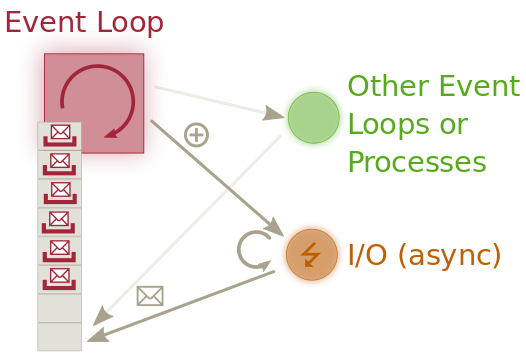
\includegraphics[scale=0.5]{./img/eventloop.png}
\end{array}$
\end{center}
\caption[Event-Loop]{Grafické znázornění Event-Loop}
\end{figure}

\subsection{Balíčkovací systém NPM}
Zejména v~posledních letech začali být velmi populární balíčkovací systémy pro různé programovací jazyky nebo frameworky inspirované balíčkovacími systémy z~operačního systému Linux respektive z~různých distribucí OS Linux. Vše začal jazyk Ruby a~především framework Ruby On Rails se~systémem tzv. Gemů. PHP dostalo balíčkovací systémy composer (aplikační moduly) a~pecl (systémové moduly). Python má pip atd,... NodeJS obsahuje svůj vlastní balíčkovací systém NPM (Node Package Manager). Disponuje velmi jenoduchům ovládáním a~přináší programátorů řešení závislostí jejich aplikací a~knihoven napříč operačními systémy.

Důležitým prvkem je konfigurační soubor \it{package.json}, obsahuje nejen informace o~závislostech programu, ale také třeba autora, verzi, popis, repozitář a~mnoho dalších údajů využívaných dalšími moduly aplikace.

Ukázkový package.json
     \begin{codeframe} 
      \begin{Verbatim}{frame=single}
{
  "name": "moje-aplikace",
  "version": "0.0.1",
  "dependencies": {
    "coffee-script": "^1.7.1",
    "express": "3.5.1",
    "mongoose": "^3.8.8",
  },
  "devDependencies": {
    "angular": "=1.2.16",
    "angular-ui-router": "^0.2.10",
  },
  "engines": {
    "node": ">=0.8.0"
  },
  "browserify": {
    "transform": [
      "coffeeify",
      "brfs",
      "envify"
    ]
  },
  "scripts": {
    "dev": "gulp dev",
    "prod": "gulp prod"
  }
}
\end{Verbatim} 
    \end{codeframe}

NPM také obsahuje interaktivný shell pro vytváření nových projektů, který vytvoří package.json za uživatele. Nově instalované moduly jsou při přidání přepínače \it{--save} nebo \it{--save-dev} přidávány také automaticky.

Základní příkazy:
\begin{description}
 \item[install] nainstaluje balíčky v package.json
 \item[install <balíček>] nainstaluje balíček
 \item[update] aktualizuje balíčky v package.json
 \item[search] vyhledávání balíčků
\end{description}

\subsection{ExpressJS}
ExpressJS je webový framework inspirovaný webovým frameworkem Synatra napsaným v ruby. Jedná se o~malý flexibilní a~robustní framework pro pro psaní single-page, multi-page a hybrodných stránek postavený na NodeJS.\cite{expressjs}
\begin{figure}[h]
\begin{center}$
\begin{array}{c}

\includegraphics[scale=0.5]{./img/express.png}
\end{array}$
\end{center}
\caption[Logo ExpressJS]{Logo ExpressJS}
\end{figure}

Express je ve stylu Synatra designován jako velmi jednoduchý a~obsahuje tak velmi malé množství funkcí, které se rozšiřuje pluginy a~knihovnami. Express tak umí především zpracovávat routy (url cesty), html požádavky (POST,GET,PUT,PATCH,OPTION) a~tělo requestů. Umí také zpracovávat a~poskytovat statické soubory a cookies.

Ukázka velmi jednoduché express aplikace:
     \begin{codeframe} 
      \begin{Verbatim}{frame=single}
express = require 'express'
server = express()
port = 3000;
router = require("./routes")

app.get "/partials/:partial", (req, res, next) ->
  res.render "assets/partials/#{req.params.partial}"

app.get "/", router.store
app.get "/editor", router.editor

app.listen port, ->
  onsole.log("Listening on #{port})
\end{Verbatim} 
    \end{codeframe}

\subsection{Mongoose ODM}
V posledních letech se stali velmi populární ORM frameworky nad MySQL databází jako je Doctrine. Pro MongoDB databázi v~prostředí NodeJS je velmi populární ODM framework Mongoose. V~MongoDB databázi neexistuje schéma jako je tomu u~SQL databází jako je MySQL. Mongoose přináší podporu pro databázové schémata validaci a~virtuální položky funkce pro práci se schématem a~rozsiřitelné API. 

Jednoduché schéma v Mongoose:
     \begin{codeframe} 
      \begin{Verbatim}{frame=single}
mongoose = require 'mongoose'
Schema = mongoose.Schema

User = new Schema
  _id:
    type: String,
  email:
    type: String
    required: true
    unique: true
    index: true
  name:
    type:String
    required:false
  address:
    city: String
  buyed_books:
    [
      type: Schema.Types.ObjectId
      ref: "Book"
    ]
  updated_at:
    type:Date
    default: Date.now
  created_at:
    type:Date
    default: Date.now

module.exports = mongoose.model 'User', User
\end{Verbatim} 
    \end{codeframe}

\section{\upc{MongoDB}}
\begin{figure}[h]
\begin{center}$
\begin{array}{c}

\includegraphics[scale=0.5]{./img/mongodb.png}
\end{array}$
\end{center}
\caption[Logo MongoDB]{Logo MongoDB}
\end{figure}
MongoDB je dokumentová NoSQL databáze s~dokumenty ve formatu json a~dynamickým schématem. Počátek jejího vývoje spadá do roku 2007 a~je vyvýjena společností 10gen, momentálně se nachází ve verzi 2.6.

MongoDB funguje jako klasický databázový server, ke kterému se klienty připojují přes síť (obvykle na portu 27017) a~komunikují s~ním speciálním protokolem (ovšem na portu 28017 najdete jednoduché HTTP rozhraní). Součástí instalace je knihovna pro C++, jako součásti projektu jsou ale vyvíjeny a~podporovány i~knihovny pro Javu, Python, Ruby, PHP a~další jazyky.

MongoDB navíc obsahuje mnoho pokročilích funkcí, jako je replikace databáze, balancování zátěže (load balancing), ukládání souborů (file storage), indexace a~další,... 

Základním rozhraním pro MongoDB je javascriptová konzole, kterou lze spustit příkazem \b{mongo}.\cite{abcLinuxuSerialMongo}

Vkládání záznamů:
     \begin{codeframe} 
      \begin{Verbatim}{frame=single}
db.users.insert(
	{
		name: "Franta",
		email: "franta@franta.cz", 
		address:{
			city:"zlín"
		}
	})
\end{Verbatim} 
	  \end{codeframe}
   
Hlednání:   
     \begin{codeframe} 
      \begin{Verbatim}{frame=single}
db.users.find()
#vrátí všechny záznamy

db.bands.find({name:"Franta"})
#vrátí záznamy se jménem Franta

db.bands.find({name: /^Fra.*/})
#regulérní výrazy v~dotazech
#vrátí všechny záznamy začínajích na Fra
\end{Verbatim} 
	  \end{codeframe}

Update:
     \begin{codeframe} 
      \begin{Verbatim}{frame=single}
db.users.update(
	{
		_id: ObjectId("4b76ef5780b71853fe6c89b6")
	}, {
		$set: {
			email: "franta@seznam.cz"
		}
	})  
\end{Verbatim} 
	  \end{codeframe}

Mazání:

     \begin{codeframe} 
      \begin{Verbatim}{frame=single}
db.users.remove({name: "Franta"})
\end{Verbatim} 
	  \end{codeframe}

reference:
     \begin{codeframe} 
      \begin{Verbatim}{frame=single}
#přidáme uživateli knihu
db.users.update(
	{
		_id: ObjectId("4b76ef5780b71853fe6c89b6")
	}, {
		$push: {
			books: new DBRef("books", ObjectId("4b7b1d6bb345126b62fb2230"))
		}
	})

#vyhledáme uživatele
db.users.findOne({_id: ObjectId("4b76ef5780b71853fe6c89b6")})
{
	"_id" : ObjectId("4b76ef5780b71853fe6c89b6"),
	"name":"Franta",
	"email":"franta@seznam.cz",
  "books" : [
          {
                  "$ref" : "books",
                  "$id" : ObjectId("4b7b1d6bb345126b62fb2230")
          }
  ],
  "address":{
		"city":"zlín"
	}
}
#získáme knihy uživatele
db.users.findOne().books.fetch()
\end{Verbatim} 
	  \end{codeframe}

\section{\upc{AngularJS}}
\begin{figure}[h]
\begin{center}$
\begin{array}{c}

\includegraphics[scale=0.5]{./img/angularjs.png}
\end{array}$
\end{center}
\caption[Logo AngularJS]{Logo AngularJS}
\end{figure}

Anglický originál popisu angularJS z repozitáře na portále github.com


\it{AngularJS lets you write client-side web applications as if you had a smarter browser. It lets you use good old HTML (or HAML, Jade and friends!) as your template language and lets you extend HTML’s syntax to express your application’s components clearly and succinctly. It automatically synchronizes data from your UI (view) with your JavaScript objects (model) through 2-way data binding. To help you structure your application better and make it easy to test, AngularJS teaches the browser how to do dependency injection and inversion of control. Oh yeah and it also helps with server-side communication, taming async callbacks with promises and deferreds; and makes client-side navigation and deeplinking with hashbang urls or HTML5 pushState a piece of cake. The best of all: it makes development fun!}\cite{angularGITHUB}

Překlad:

\it{AngularJS vám umožní vytvářet tenké klientské aplikace, jakobyste měli chytřejší prohlížeč. Přitom můžete používat staré známé HTML (HAML, JADE a~podobné) jako šablonovací systém a~rozšířit jeho syntaxy tak aby komponenty vyjadřovali aplikaci jasně a~stručně. Automaticky synchornizuje data v~uživatelském rozhraní s~vaším javascriptovým modelem, pomocí obousměrné datové vazby. Abyste mohli strukturovat vaši aplikaci lépe a~udělali ji snáze testovatelnou, AngularJS učí váš prohlížeč jak na devendency injection a~inversion of~control. A abych nezapomněl také vám pomůže s~komunikací se serverem, pomůže vám zkrotit asynchroní callbacky, promises a~deferreds; a~také dělá navigaci v~prohlížeči, pomocí deeplinking s~hashbang url nebo html5 pushState snadnou věcí. A to nejlepší na konec: dělá vývoj webových aplikací zábavou.}\cite{angularGITHUB}

\subsection{Struktura}
Struktura kódu aplikace by měla mít nějaká pravidla, tak aby se v~kódu vyznam i~někdo jiný než autor samotný. Proto napříkal google poskytuje online doporučenou strukturu kódu pro aplikace napsané v~AngularJS. Online verze je dostupná na adrese: \href{https://google-styleguide.googlecode.com/svn/trunk/angularjs-google-style.html}{https://google-styleguide.googlecode.com/svn/trunk/angularjs-google-style.html}
\it{Vzhledem k tomu,že se jedná o~obsáhlejší dokument nebude nijak komentován. Ale struktura aplikace je z~větší části ovlivněna právě tímto návrhem.}

Co se týče struktury adresářové, existuje zde několik návrhů, které jsou určeny pro různě velké aplikace.

Velmi jednoduchá aplikace v~AngularJS vypadá nějak takto:
     \begin{codeframe} 
      \begin{Verbatim}{frame=single}
css/
img/
js/
	app.js
	controllers.js
	directives.js
	filters.js
	services.js
lib/
partials/
\end{Verbatim} 
	  \end{codeframe}
Vše je rozděleno do několika javascriptových souborů, které reprezentují jednotlivé moduly AngularJS, je to o~něco málo lepší, než jednosouborové aplikace tak jak to dělá velké množství uživatelů jQuery, ale jednotlivé soubory nereprezentují konkrétní funkcionalitu, takže se v projektu hůře orientuje.\cite{angularJSFolders}

Tento problém řeší rozdělení jednotlivých modulů do několika sub-modulů, které již reprezentují svoji funkcionalitu.
     \begin{codeframe} 
      \begin{Verbatim}{frame=single}
controllers/
	LoginController.js
	RegistrationController.js
	ProductDetailController.js
	SearchResultsController.js
common/
	cartDirective.js
	productFilter.js
models/
	CartModel.js
	ProductModel.js
	SearchResultsModel.js
	UserModel.js
services/
	CartService.js
	UserService.js
	ProductService.js
\end{Verbatim} 
	  \end{codeframe}

V~případě, že vytvářím, větší aplikaci, stane se pro mě toto schéma také nedostatečným, protože ve větších aplikacích už je většinou třeba shlukovat veškeré části dané funkcionality u~sebe, takže ještě je třeba strukturu ještě přeskupit.
     \begin{codeframe} 
      \begin{Verbatim}{frame=single}
cart/
	index.less
	CartModel.js
	CartService.js
common/
	cartDirective.js
	productFilter.js
product/
	search/
		SearchResultsController.js
		SearchResultsModel.js
	ProductDetailController.js
	ProductModel.js
	ProductService.js
	index.less
	show.html
user/
	show.html
	edit.html
	index.less
	LoginController.js
	RegistrationController.js
	UserModel.js
	UserService.js
\end{Verbatim} 
	  \end{codeframe}

\subsection{Router}
Router je další důležitá přednost AngularJS, jak už bylo v úvodu zmíněno routování umožňuje přepínat mezi url hashangem a~html5.pushState. Router v AngularJS je navíc modulem, který lze vyměnit takže můžeme místo něj použít třeba ui-router, který jeden z~nejpoužívanějších modulů pro AngularJS. Oproti angular-routeru je ui-router stavový, takže každá změna ui může být reprezentována svým stanem, který můze být jednoduše vnořen a~výsledkem je pak přehledná hierarchie routeru a~url.

Ukázka jednoduché routeru v~modulu angular-router
     \begin{codeframe} 
      \begin{Verbatim}{frame=single}
phonecatApp.config [
  "$routeProvider"
  ($routeProvider) ->
    $routeProvider.when("/phones",
      templateUrl: "partials/phone-list.html"
      controller: "PhoneListCtrl"
    ).when("/phones/:phoneId",
      templateUrl: "partials/phone-detail.html"
      controller: "PhoneDetailCtrl"
    ).otherwise redirectTo: "/phones"
]
\end{Verbatim} 
	  \end{codeframe}

Ukázka ui-router
     \begin{codeframe} 
      \begin{Verbatim}{frame=single}
phonecatApp.config [
  "$stateProvider, $urlRouterProvider",
  ($stateProvider, $urlRouterProvider) ->
    $urlRouterProvider.otherwise "/phones"
    $stateProvider.state("phones",
      url: "/phones"
      templateUrl: "partials/phones-list.html"
    ).state("phones.one",
      url: "/:id"
      templateUrl: "partials/phone-detail.list.html"
      controller: "PhoneDetailCtrl"
    )
]
\end{Verbatim} 
	  \end{codeframe}
Z ukázky je vidět, že stavy v~ui-routeru, jsou hierarchycké a lépe se v~nich orientuje.

\subsection{Controller}
\subsection{Directive}
\subsection{Factory}
\subsection{Filter}
\subsection{Animation}
\subsection{Value}

\section{\upc{LESS}}
\begin{figure}[h]
\begin{center}$
\begin{array}{c}

\includegraphics[scale=0.5]{./img/less.png}
\end{array}$
\end{center}
\caption[Logo Less]{Logo Less}
\end{figure}

\section{\upc{JADE}}
\begin{figure}[h]
\begin{center}$
\begin{array}{c}

\includegraphics[scale=0.5]{./img/jade.png}
\end{array}$
\end{center}
\caption[Logo Jade]{Logo Jade}
\end{figure}

\section{\upc{Bower}}
\begin{figure}[h]
\begin{center}$
\begin{array}{c}

\includegraphics[scale=0.5]{./img/bower.png}
\end{array}$
\end{center}
\caption[Logo Less]{Logo Less}
\end{figure}

\section{\upc{GulpJS}}
\begin{figure}[h]
\begin{center}$
\begin{array}{c}

\includegraphics[scale=0.5]{./img/gulp.png}
\end{array}$
\end{center}
\caption[Logo GulpJS]{Logo GulpJS}
\end{figure}

% \begin{figure}[h]
% \begin{center}$
% \begin{array}{c}
% 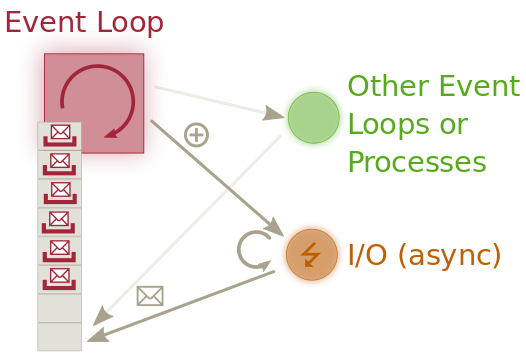
\includegraphics[scale=0.5]{./img/eventloop.png}
% \end{array}$
% \end{center}
% \caption[Grafické znázornění Event-Loop]{}
% \end{figure}


% \begin{description}
%  \item[ITEM] TEXT
%  \end{description}

% \subsubsection{subsub}

% \begin{itemize}
%  \item LFS učí uživatele, jak Linux funguje uvnitř.
% \end{itemize}
% \begin{enumerate}
% \item ITEM
% \end{enumerate}


% \nadpis{Remastersys}

% \nadpis{The Ubuntu Customisation Kit (UCK)}\\ \label{sec:UCK}
% \odkazNaKapitolu{sec:UCK}\\

% \begin{figure}[h]
% \begin{center}$
% \begin{array}{cc}
% 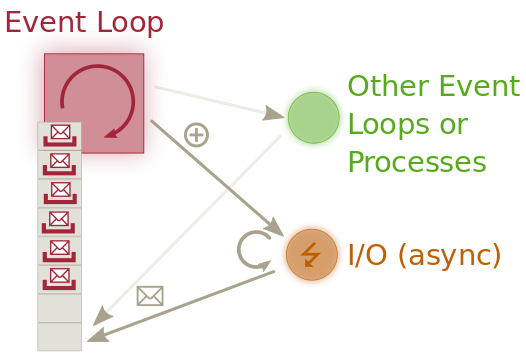
\includegraphics[scale=0.5]{./img/eventloop.png} &
% 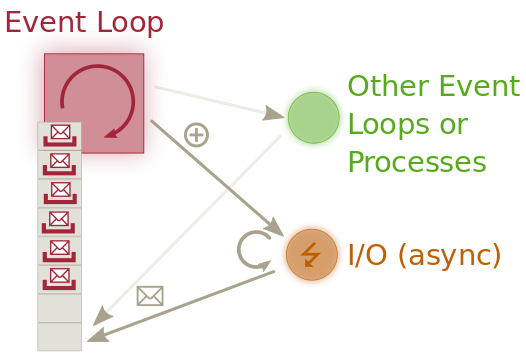
\includegraphics[scale=0.5]{./img/eventloop.png}
% \end{array}$
% \end{center}
% \caption[Webové rozhraní Instalinux, distribuce/časová zóna]{Webové rozhraní Instalinux, vlevo výběr distribuce, vpravo nastavení jazyka a~časové zóny}
% \end{figure}

\newpage

\vspace{4 mm}


%********************************* Analytická část ************************************
%\part{Analytická část}
%\sectionV{Nadpis}
%\subsection{Podnadpis}
%********************************* Projektová část ************************************
\part{Projektová část}
\section{\upc{Funkcionalita}}
\section{\upc{Rozšíření a návrhy}}


\section{\upc{Databáze}}
\subsection{Návrh/schéma}
\subsection{Budoucí vývoj}
\subsection{Zabezpečení}
\subsection{Nasazení (server,cloud)}

\section{\upc{Backend}}
\subsection{Struktura}
\subsection{API}
\subsection{Zabezpečení}
\subsubsection{Server}
\subsubsection{Kontejner}
\subsection{Přihlášení a soukromí uživatelů}
\subsection{ACL}

\section{\upc{Frontend}}
\subsection{Struktura}
\subsection{Komponenty}

\subsubsection{Store (e-shop)}
\subsubsection{Create (správa vlastních knih)}
\subsubsection{Edit (editor knih)}
\subsubsection{Finance}
\subsubsection{Storage (pobočky a sklady)}
\subsubsection{Statistics (statistiky)}
\subsubsection{Admin (administrace)}


\section{\upc{Gulp}}


%********************************* Závěr ************************************
\nn{Závěr}
Cílem této bakalářské práce bylo vytvořit sadu skriptů v~jazyce BASH pro automatické sestavení Linuxové distribuce Linux From Scratch. Pro návrh skriptů byl použit návod pro sestavení distribuce Linux From Scratch a~nemalou měrou přispěl i~verzovací systém GIT a~komunitní web pro správu git repozitářů GitHub.\\

V~teoretické části bylo provedeno seznámení s~Linuxem, jeho distribucemi a~možnostmi tvorby distribucí včetně kompilace zdrojových kódů a~programování v~interpretovaném jazyce BASH, což~jsou důležité znalosti pro vytvoření distribuce Linuxu. Dále bylo provedeno seznámení se zabezpečením Linuxu a~systémem hodnocení bezpečnosti Softwaru. Praktická část byla věnována skriptům v~interpretovaném jazyce BASH, jejich struktuře, obsahu a~návodu pro použití. Skripty byly otestovány jak na virtuálním počítači, vytvořeného programem VirtualBox a~s~použitím systému Ubuntu 10.10 Maverick Meerkat, tak na fyzickém počítači se~systémem ArchLinux.\\

Programování v~interpretovaném jazyce BASH je velmi zajímavé, zvláště vzhledem k~jeho integraci se systémem Linux. Jsem rád, že~jsem si mohl rozšířit prostřednictvím této bakalářské práce znalosti tohoto jazyka, o~tomto svědčí i~fakt, že jsem dvakrát přepsal způsob jakým skripty fungují. Také jsem rozšířil své znalosti o~tom jak funguje Operační systém Linux v~širším měřítku, za~což jsem velmi rád.
%********************************* Závěr anglicky************************************
\newpage
\nn{Závěr v Angličtině}
The aim of this bachelor work was to~create a~set of~BASH scripts for~automatic compilation Linux From Scratch distribution. For the~design of~scripts was used Linux From Scratch book and~in~no small part contributed GIT version control system and community site for managing git repositories GitHub. 

In the theoretical part was made introduction with Linux, the~Linux distributions and creation of~Linux distributions, including a~compilation of~source code and~programming interpreted language BASH, which are~important skills for~a~building Linux distribution. It~was also made familiar with~the~security of~Linux and~system software safety assessment. The~practical part was devoted to~scripts in~BASH, its structure, contents and~instructions for~use. Scripts was~tested in~virtual computer created by~program VirtualBox and~runing Ubuntu 10.10 Meerkat Maverick, and~at~the~physical computer running ArchLinux. 

Programming in interpreted language BASH is very interesting, especially due to integration with Linux. I'm glad that I was able to extend my knowledge of~BASH becouse of this work. True of that was demonstrated by the fact that I'm twice rewrote the way how the script works. I also expanded my knowledge about the functioning of the Linux operating system on a larger scale, for which I am very happy.

\newpage
%********************************* Seznam Literatury ************************************
\seznamlit{
\bibitem{nodejsEventArch}http://www.nodejs.cz/co-je-event-driven-architektura/. [e-kniha] 
\bibitem{expressjs}http://expressjs.com/. [e-kniha] 
\bibitem{abcLinuxuSerialMongo}http://www.abclinuxu.cz/clanky/programovani/lehky-uvod-do-mongodb. [e-kniha] 
\bibitem{angularGITHUB}https://github.com/angular/angular.js. [e-kniha] 
\bibitem{angularJSFolders}http://cliffmeyers.com/blog/2013/4/21/code-organization-angularjs-javascript. [e-kniha] 
\bibitem{BASHen}http://www.nodejs.cz/co-je-event-driven-architektura/. [e-kniha] 
}

%********************************* Seznam zkratek ************************************
\seznamzkr

\begin{tabular}{ll}
LFS & Linux From Scratch \\
\end{tabular}
%********************************* Seznam obrázků ************************************
\seznamobr
%********************************* Seznam tabulek ************************************
%\seznamtab
%********************************* Seznam příloh ************************************
\listofappendices

\priloha{PDF verze bakalářské práce a zdrojový kód v~jazyce LaTeX}

PDF je dostupné na DVD v~portále STAG a~na~internetu\\

\href{https://github.com/zajca/BC.TvorbaLinuxoveDistribuce}{https://github.com/zajca/BC.TvorbaLinuxoveDistribuce}\\


%\section*{PŘÍLOHA P I: ŠABLONA SLOVNĚ.}
\end{document}
